% ============================================================
%  LeJEPA Presentation Slides
%  Compile with: xelatex slides.tex  (for Vietnamese support)
%  Or:           pdflatex slides.tex (English/math only)
% ============================================================
\documentclass[aspectratio=169,12pt]{beamer}

% ---------- Theme ----------
\usetheme{Madrid}
\usecolortheme{default}
\setbeamertemplate{navigation symbols}{}
\setbeamertemplate{footline}[frame number]
\setbeamertemplate{itemize items}[circle]

% ---------- Encoding (pdflatex) ----------
\usepackage[utf8]{inputenc}
\usepackage[T1]{fontenc}
\usepackage{lmodern}

% ---------- Math ----------
\usepackage{amsmath,amssymb,amsthm}
\usepackage{bm}

% ---------- Graphics ----------
\usepackage{tikz}
\usepackage{pgfplots}
\pgfplotsset{compat=1.18}
\usetikzlibrary{
  arrows.meta, positioning, shapes.geometric, shapes.misc,
  fit, backgrounds, decorations.pathreplacing,
  calc, matrix, chains, scopes
}

% ---------- Tables ----------
\usepackage{booktabs}
\usepackage{colortbl}
\usepackage{multirow}
\usepackage{array}

% ---------- Strikethrough & Symbols ----------
\usepackage[normalem]{ulem}
\usepackage{pifont}
\newcommand{\cmark}{\ding{51}}
\newcommand{\xmark}{\ding{55}}

% ---------- Code ----------
\usepackage{listings}
\lstset{
  basicstyle=\ttfamily\tiny,
  keywordstyle=\color{primary}\bfseries,
  commentstyle=\color{neutral},
  backgroundcolor=\color{black!5},
  frame=single, framerule=0pt,
  breaklines=true, language=Python
}

% ---------- Colors ----------
\definecolor{primary}{HTML}{1E40AF}
\definecolor{accent}{HTML}{F59E0B}
\definecolor{bad}{HTML}{DC2626}
\definecolor{good}{HTML}{10B981}
\definecolor{neutral}{HTML}{6B7280}
\definecolor{lightblue}{HTML}{DBEAFE}
\definecolor{lightyellow}{HTML}{FEF3C7}
\definecolor{lightgreen}{HTML}{D1FAE5}
\definecolor{lightred}{HTML}{FEE2E2}
\definecolor{lightgray}{HTML}{F3F4F6}

\setbeamercolor{structure}{fg=primary}
\setbeamercolor{alerted text}{fg=accent}
\setbeamercolor{block title}{bg=primary, fg=white}
\setbeamercolor{block body}{bg=lightblue}
\setbeamercolor{block title alerted}{bg=bad, fg=white}
\setbeamercolor{block body alerted}{bg=lightred}
\setbeamercolor{block title example}{bg=good, fg=white}
\setbeamercolor{block body example}{bg=lightgreen}

% ---------- Helpers ----------
\newcommand{\takeaway}[1]{%
  \vfill
  \begin{beamercolorbox}[sep=4pt,center,rounded=true]{block title alerted}
    \small\bfseries #1
  \end{beamercolorbox}
}
\newcommand{\good}[1]{\textcolor{good}{#1}}
\newcommand{\bad}[1]{\textcolor{bad}{#1}}
\newcommand{\hl}[1]{\textcolor{accent}{\bfseries #1}}

% ============================================================
\title[LeJEPA]{\textbf{LeJEPA}: Provable \& Scalable\\
Self-Supervised Learning Without the Heuristics}
\author{Randall Balestriero \& Yann LeCun (2025)}
\institute{arXiv: 2511.08544}
\date{}
% ============================================================

\begin{document}

% ============================================================
%  SLIDE 1 — Title
% ============================================================
\begin{frame}
\begin{columns}[c]
\column{0.55\textwidth}
  \vspace{0.5cm}
  {\Large\bfseries\color{primary} LeJEPA}\\[4pt]
  {\normalsize Provable \& Scalable SSL\\Without the Heuristics}\\[12pt]
  {\small Randall Balestriero \& Yann LeCun (2025)\\
  \texttt{arXiv: 2511.08544}}\\[16pt]
  {\footnotesize Presenter: [Ten ban]}

\column{0.43\textwidth}
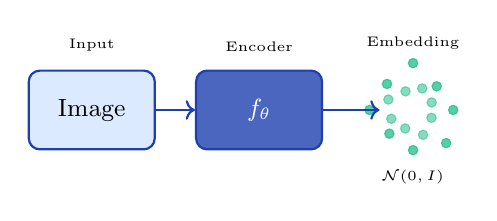
\begin{tikzpicture}[scale=0.85]
  % Pipeline: Image -> Encoder -> N(0,I)
  \node[draw=primary, thick, rounded corners=4pt, fill=lightblue,
        minimum width=1.6cm, minimum height=1cm] (img) at (0,0)
        {\small Image};
  \node[draw=primary, thick, rounded corners=4pt, fill=primary!80,
        text=white, minimum width=1.6cm, minimum height=1cm] (enc) at (2.5,0)
        {\small $f_\theta$};
  % Gaussian dots
  \begin{scope}[shift={(4.8,0)}]
    \foreach \a/\r in {0/0.6, 45/0.5, 90/0.7, 135/0.55, 180/0.65,
                        225/0.5, 270/0.6, 315/0.7}
      \filldraw[good, opacity=0.7]
        ({cos(\a)*\r},{sin(\a)*\r}) circle (2pt);
    \foreach \a/\r in {22/0.3, 67/0.35, 112/0.3, 157/0.4,
                        202/0.35, 247/0.3, 292/0.4, 337/0.3}
      \filldraw[good, opacity=0.5]
        ({cos(\a)*\r},{sin(\a)*\r}) circle (2pt);
    \node at (0,-1) {\tiny $\mathcal{N}(0,I)$};
  \end{scope}
  \draw[->, thick, primary] (img) -- (enc);
  \draw[->, thick, primary] (enc) -- (4.3,0);
  % Labels
  \node[above=3pt of img] {\tiny Input};
  \node[above=3pt of enc] {\tiny Encoder};
  \node at (4.8,1) {\tiny Embedding};
\end{tikzpicture}
\end{columns}
\end{frame}

% ============================================================
%  SLIDE 2 — Overview (table of contents style)
% ============================================================
\begin{frame}{Outline}
\begin{columns}[t]
\column{0.48\textwidth}
\begin{block}{Part 1: Background}
\begin{enumerate}\small
  \item Ba cach AI hoc tu du lieu
  \item Van de collapse trong SSL
  \item JEPA: y tuong co ban
  \item Cac phuong phap hien tai: han che
\end{enumerate}
\end{block}
\vspace{6pt}
\begin{block}{Part 2: Theory}
\begin{enumerate}\setcounter{enumi}{4}\small
  \item Distribution nao la optimal?
  \item Linear probe: iso beats aniso
  \item Nonlinear probe: iso Gaussian unique
  \item Geometric intuition
\end{enumerate}
\end{block}

\column{0.48\textwidth}
\begin{block}{Part 3: SIGReg}
\begin{enumerate}\setcounter{enumi}{8}\small
  \item Thu thach high-dim testing
  \item 1D Slicing (Cramer-Wold)
  \item So sanh 3 ho test 1D
  \item Epps-Pulley: bounded gradient
  \item SIGReg: cong thuc cuoi
\end{enumerate}
\end{block}
\vspace{6pt}
\begin{block}{Part 4--7: LeJEPA + Results + Impact}
\begin{enumerate}\setcounter{enumi}{13}\small
  \item Pipeline hoan chinh
  \item So sanh DINO/I-JEPA
  \item Ket qua tren 60+ kien truc
  \item Impact \& citation
\end{enumerate}
\end{block}
\end{columns}
\end{frame}

% ============================================================
%  SLIDE 3 — Ba paradigm
% ============================================================
\begin{frame}{Ba Paradigm: AI Hoc Nhu The Nao?}
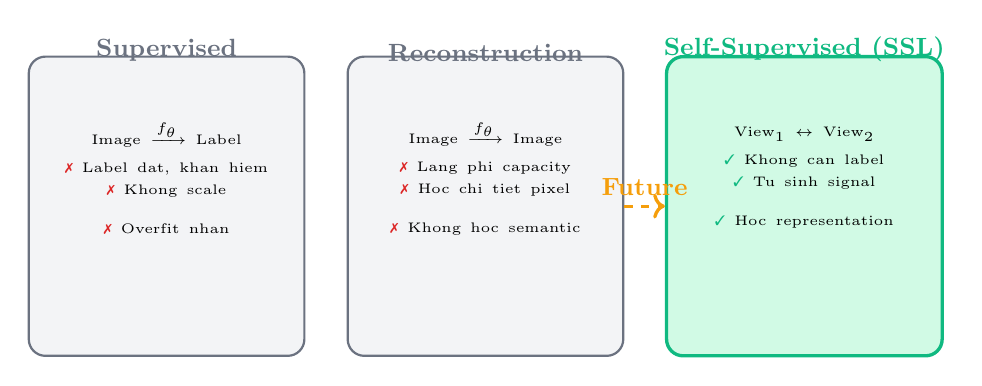
\begin{tikzpicture}[scale=0.9]
  % Box Supervised
  \node[draw=neutral, thick, rounded corners=6pt, fill=lightgray,
        minimum width=3.5cm, minimum height=3.8cm,
        text width=3.2cm, align=center] (sup) at (0,0) {};
  \node[above] at (0,1.9) {\small\bfseries\color{neutral} Supervised};
  \node[align=center, text width=3cm] at (0,0.4)
    {\tiny Image $\xrightarrow{f_\theta}$ Label\\[4pt]
     \bad{\ding{55}} Label dat, khan hiem\\[2pt]
     \bad{\ding{55}} Khong scale\\[2pt]
     \bad{\ding{55}} Overfit nhan};

  % Box Reconstruction
  \node[draw=neutral, thick, rounded corners=6pt, fill=lightgray,
        minimum width=3.5cm, minimum height=3.8cm,
        text width=3.2cm, align=center] (rec) at (4.5,0) {};
  \node[above] at (4.5,1.9) {\small\bfseries\color{neutral} Reconstruction};
  \node[align=center, text width=3cm] at (4.5,0.4)
    {\tiny Image $\xrightarrow{f_\theta}$ Image\\[4pt]
     \bad{\ding{55}} Lang phi capacity\\[2pt]
     \bad{\ding{55}} Hoc chi tiet pixel\\[2pt]
     \bad{\ding{55}} Khong hoc semantic};

  % Box SSL
  \node[draw=good, very thick, rounded corners=6pt, fill=lightgreen,
        minimum width=3.5cm, minimum height=3.8cm,
        text width=3.2cm, align=center] (ssl) at (9,0) {};
  \node[above] at (9,1.9) {\small\bfseries\color{good} Self-Supervised (SSL)};
  \node[align=center, text width=3cm] at (9,0.4)
    {\tiny View$_1$ $\leftrightarrow$ View$_2$\\[4pt]
     \good{\ding{51}} Khong can label\\[2pt]
     \good{\ding{51}} Tu sinh signal\\[2pt]
     \good{\ding{51}} Hoc representation};

  % Arrow highlight
  \draw[->, very thick, accent, dashed] (rec.east) -- (ssl.west)
    node[midway, above, accent, font=\small\bfseries] {Future};
\end{tikzpicture}
\vspace{6pt}
\takeaway{SSL: AI hoc tu cau truc du lieu, khong phu thuoc nhan con nguoi}
\end{frame}

% ============================================================
%  SLIDE 4 — Representation Collapse
% ============================================================
\begin{frame}{Van De Cot Loi: Representation Collapse}
\begin{columns}[c]
\column{0.48\textwidth}
\begin{center}
\textbf{\bad{Trivial Solution (Collapse)}}\\[6pt]
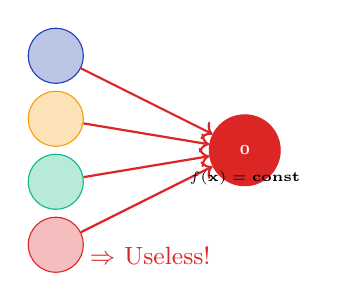
\begin{tikzpicture}[scale=0.8]
  % Input nodes
  \foreach \y/\c in {2/primary, 1/accent, 0/good, -1/bad}
    \node[circle, draw=\c, fill=\c!30, minimum size=0.7cm] (in\y) at (0,\y) {};
  % Single output
  \node[circle, draw=bad, fill=bad, minimum size=0.9cm,
        text=white, font=\tiny] (out) at (3,0.5) {$\mathbf{0}$};
  % Arrows
  \foreach \y in {2,1,0,-1}
    \draw[->, bad, thick] (in\y) -- (out);
  \node[below=4pt] at (out) {\tiny $f(\mathbf{x}) = \mathbf{const}$};
  \node[below=20pt] at (1.5,0) {\small \bad{$\Rightarrow$ Useless!}};
\end{tikzpicture}
\end{center}

\column{0.48\textwidth}
\begin{center}
\textbf{\good{Desired: Rich Embeddings}}\\[6pt]
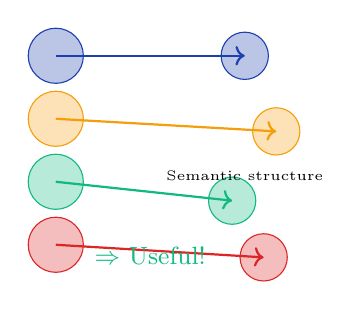
\begin{tikzpicture}[scale=0.8]
  % Input nodes
  \foreach \y/\c in {2/primary, 1/accent, 0/good, -1/bad}
    \node[circle, draw=\c, fill=\c!30, minimum size=0.7cm] (in\y) at (0,\y) {};
  % Different output points
  \node[circle, draw=primary, fill=primary!30, minimum size=0.6cm] at (3,2) {};
  \node[circle, draw=accent, fill=accent!30, minimum size=0.6cm] at (3.5,0.8) {};
  \node[circle, draw=good, fill=good!30, minimum size=0.6cm] at (2.8,-0.3) {};
  \node[circle, draw=bad, fill=bad!30, minimum size=0.6cm] at (3.3,-1.2) {};
  % Arrows
  \draw[->, primary, thick] (0,2) -- (3,2);
  \draw[->, accent, thick] (0,1) -- (3.5,0.8);
  \draw[->, good, thick] (0,0) -- (2.8,-0.3);
  \draw[->, bad, thick] (0,-1) -- (3.3,-1.2);
  \node[below=4pt] at (3,0.5) {\tiny Semantic structure};
  \node[below=20pt] at (1.5,0) {\small \good{$\Rightarrow$ Useful!}};
\end{tikzpicture}
\end{center}
\end{columns}
\vspace{4pt}
\begin{alertblock}{Two types of collapse}
\small
\textbf{Complete:} $f(\mathbf{x}) = \mathbf{c}$ for all $\mathbf{x}$ \quad
\textbf{Dimensional:} all embeddings lie on a low-dim subspace
\end{alertblock}
\takeaway{Prediction objective alone $\Rightarrow$ trivial solution: $\min\|f(v_1)-f(v_2)\|=0$}
\end{frame}

% ============================================================
%  SLIDE 5 — JEPA
% ============================================================
\begin{frame}{JEPA: Joint-Embedding Predictive Architecture (LeCun, 2022)}
\begin{columns}[c]
\column{0.55\textwidth}
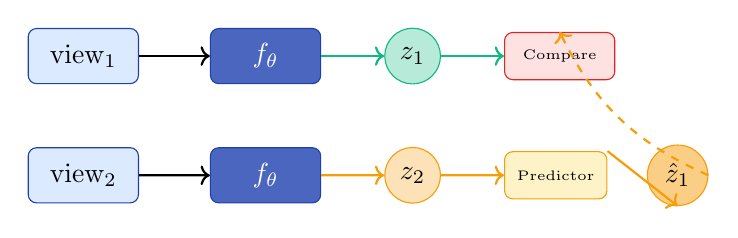
\begin{tikzpicture}[node distance=1.2cm, scale=0.85]
  % Views
  \node[draw=primary, fill=lightblue, rounded corners=3pt,
        minimum width=1.4cm, minimum height=0.7cm] (v1) {view$_1$};
  \node[draw=primary, fill=lightblue, rounded corners=3pt,
        minimum width=1.4cm, minimum height=0.7cm, below=0.8cm of v1] (v2) {view$_2$};
  % Encoders
  \node[draw=primary, fill=primary!80, text=white, rounded corners=3pt,
        minimum width=1.4cm, minimum height=0.7cm, right=0.9cm of v1] (e1) {$f_\theta$};
  \node[draw=primary, fill=primary!80, text=white, rounded corners=3pt,
        minimum width=1.4cm, minimum height=0.7cm, right=0.9cm of v2] (e2) {$f_\theta$};
  % Embeddings
  \node[circle, draw=good, fill=good!30, minimum size=0.6cm,
        right=0.8cm of e1] (z1) {$z_1$};
  \node[circle, draw=accent, fill=accent!30, minimum size=0.6cm,
        right=0.8cm of e2] (z2) {$z_2$};
  % Predictor
  \node[draw=accent, fill=lightyellow, rounded corners=3pt,
        minimum width=1.3cm, minimum height=0.6cm, right=0.8cm of z2] (pred) {\tiny Predictor};
  \node[circle, draw=accent, fill=accent!50, minimum size=0.6cm,
        above=0.3cm of pred, right=0.5cm of pred] (zhat) {$\hat{z}_1$};
  % Compare
  \node[draw=bad, fill=lightred, rounded corners=3pt,
        minimum width=1.4cm, minimum height=0.6cm, right=0.8cm of z1] (cmp) {\tiny Compare};
  % Arrows
  \draw[->, thick] (v1) -- (e1);
  \draw[->, thick] (v2) -- (e2);
  \draw[->, thick, good] (e1) -- (z1);
  \draw[->, thick, accent] (e2) -- (z2);
  \draw[->, thick, accent] (z2) -- (pred);
  \draw[->, thick, accent] (pred.north east) -- (zhat.south);
  \draw[->, thick, good] (z1) -- (cmp);
  \draw[->, thick, accent, dashed] (zhat.east) to[bend left=20] (cmp.north);
\end{tikzpicture}

\column{0.42\textwidth}
\begin{block}{2 Nguyen Tac JEPA}
\begin{enumerate}\small
  \item \textbf{Predictability:}\\
  $\text{Enc}(\mathbf{x}_{t+1})$ predictable\\
  from $\text{Enc}(\mathbf{x}_t)$
  \vspace{4pt}
  \item \textbf{Non-degeneracy:}\\
  Embeddings khong\\
  duoc collapse
\end{enumerate}
\end{block}
\vspace{6pt}
\begin{exampleblock}{Khac LLM}
\small JEPA predict \textbf{abstract state}\\
(embedding space)\\
$\neq$ predict pixel/token\\
$\Rightarrow$ Bo qua chi tiet nhieu
\end{exampleblock}
\end{columns}
\takeaway{JEPA hoc ``the gioi thay doi the nao'', khong hoc ``pixel trong nhu the nao''}
\end{frame}

% ============================================================
%  SLIDE 6 — Whac-A-Mole (current methods)
% ============================================================
\begin{frame}{Cac Phuong Phap Hien Tai: Heuristic Stack}
\begin{center}
\begin{tabular}{llll}
\toprule
\textbf{Method} & \textbf{Co che chong collapse} & \textbf{Limitation chinh} \\
\midrule
SimCLR  & Negative samples (contrastive)
        & \cellcolor{lightred}$\mathcal{O}(N^2)$ memory \\[2pt]
BYOL    & Asymmetric arch + stop-gradient
        & \cellcolor{lightred}No theory, brittle \\[2pt]
DINO    & Teacher--student + EMA schedule
        & \cellcolor{lightred}$\geq$7 hyperparameters \\[2pt]
VICReg  & Variance/covariance whitening
        & \cellcolor{lightred}Under-specified \\[2pt]
I-JEPA  & Stop-gradient + mask prediction
        & \cellcolor{lightred}ViT-only, sensitive \\
\bottomrule
\end{tabular}
\end{center}
\vspace{6pt}
\begin{columns}[t]
\column{0.48\textwidth}
\begin{alertblock}{4 Han Che Chung}
\footnotesize
\begin{enumerate}
  \item \textbf{Under-specified:} co the minimize loss ma van degenerate
  \item \textbf{$\mathcal{O}(N^2)$:} khong scale len batch lon
  \item \textbf{Nhay HP:} doi architecture $\to$ collapse
  \item \textbf{No theory:} khong biet tai sao work
\end{enumerate}
\end{alertblock}
\column{0.48\textwidth}
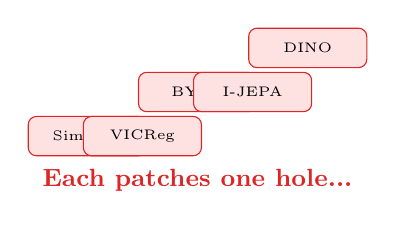
\begin{tikzpicture}[scale=0.7]
  % Whac-a-mole metaphor
  \foreach \x/\t in {0/SimCLR, 2/BYOL, 4/DINO, 1/VICReg, 3/I-JEPA}
    \node[draw=bad, fill=lightred, rounded corners=3pt,
          minimum width=1.5cm, minimum height=0.5cm,
          font=\tiny] at (\x, {int(\x/2)*0.8}) {\t};
  \node[font=\small\bfseries\color{bad}] at (2,-0.8) {Each patches one hole...};
\end{tikzpicture}
\end{columns}
\takeaway{Khong co framework nao xuat phat tu first principles --- chi la empirical patches}
\end{frame}

% ============================================================
%  SLIDE 7 — The pivot question
% ============================================================
\begin{frame}{Cau Hoi Thay Doi Moi Thu}
\begin{columns}[c]
\column{0.48\textwidth}
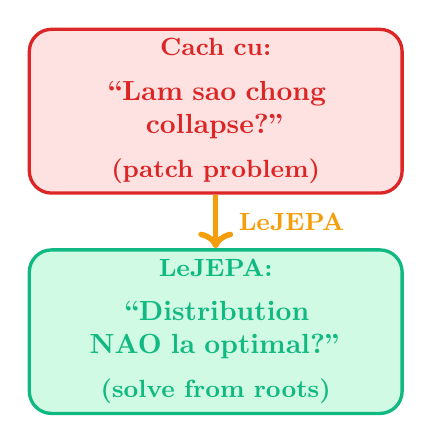
\begin{tikzpicture}
  \node[draw=bad, very thick, rounded corners=8pt, fill=lightred,
        text width=4.5cm, align=center, minimum height=1.8cm] (old) at (0,0)
    {\small\bfseries\color{bad} Cach cu:\\[4pt]
     \normalsize ``Lam sao chong collapse?''\\[4pt]
     \small (patch problem)};
  \node[draw=good, very thick, rounded corners=8pt, fill=lightgreen,
        text width=4.5cm, align=center, minimum height=1.8cm] (new) at (0,-2.8)
    {\small\bfseries\color{good} LeJEPA:\\[4pt]
     \normalsize ``Distribution NAO la optimal?''\\[4pt]
     \small (solve from roots)};
  \draw[->, very thick, accent, line width=2pt] (old) -- (new)
    node[midway, right=4pt, accent, font=\small\bfseries] {LeJEPA};
\end{tikzpicture}

\column{0.48\textwidth}
\begin{block}{2 Axioms cua LeJEPA}
\begin{enumerate}
  \item Solve the prediction task\\
  {\footnotesize (standard practice)}
  \vspace{4pt}
  \item Enforce \textbf{isotropic Gaussian}\\
  distribution of embeddings\\
  {\footnotesize (NEW --- proven optimal)}
\end{enumerate}
\end{block}
\vspace{8pt}
\begin{exampleblock}{Key Insight}
\small Neu biet distribution nao toi uu $\to$ thiet ke loss nham thang toi do\\
$\to$ collapse tu giai quyet
\end{exampleblock}
\end{columns}
\takeaway{Doi tu ``prevent collapse'' sang ``achieve optimal distribution''}
\end{frame}

% ============================================================
%  SLIDE 8 — Linear Probe Setup
% ============================================================
\begin{frame}{Setup: Danh Gia Qua Linear Probe}
\begin{columns}[c]
\column{0.52\textwidth}
\begin{block}{Ridge Regression (OLS)}
\[
\hat{\beta} = \underset{\beta}{\arg\min}
\|\mathbf{y} - \mathbf{Z}\beta\|_2^2 + \lambda\|\beta\|_2^2
\]
\end{block}
\vspace{6pt}
\textbf{Cau hoi:} Distribution cua $\mathbf{Z}$ nao giup uoc luong $\beta$ tot nhat?
\vspace{8pt}

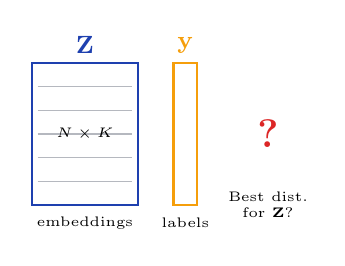
\begin{tikzpicture}[scale=0.75]
  % Matrix Z
  \draw[primary, thick] (0,0) rectangle (1.8,2.4);
  \node[primary, font=\small\bfseries] at (0.9,2.7) {$\mathbf{Z}$};
  \foreach \y in {0.4,0.8,1.2,1.6,2.0}
    \draw[neutral!50] (0.1,\y) -- (1.7,\y);
  \node[font=\tiny] at (0.9,1.2) {$N\times K$};
  \node[font=\tiny] at (0.9,-0.3) {embeddings};
  % Vector y
  \draw[accent, thick] (2.4,0) rectangle (2.8,2.4);
  \node[accent, font=\small\bfseries] at (2.6,2.7) {$\mathbf{y}$};
  \node[font=\tiny] at (2.6,-0.3) {labels};
  % Question mark
  \node[font=\Large\bfseries\color{bad}] at (4,1.2) {?};
  \node[font=\tiny, align=center] at (4,0) {Best dist.\\for $\mathbf{Z}$?};
\end{tikzpicture}

\column{0.44\textwidth}
\textbf{Hai ung vien (cung energy):}
\vspace{6pt}


\begin{tikzpicture}[scale=0.7]
  % Anisotropic
  \begin{scope}
    \draw[bad, thick] (0,0) ellipse (1.5cm and 0.5cm);
    \foreach \a in {0,30,...,330}
      \filldraw[bad!70] ({1.4*cos(\a)},{0.45*sin(\a)}) circle (2pt);
    \node[bad, font=\footnotesize\bfseries] at (0,-0.9) {Anisotropic};
    \node[font=\tiny, bad] at (0,-1.3) {$\lambda_1 \neq \lambda_2$};
  \end{scope}
  % Isotropic
  \begin{scope}[shift={(4,0)}]
    \draw[good, thick] (0,0) circle (0.9cm);
    \foreach \a in {0,30,...,330}
      \filldraw[good!70] ({0.85*cos(\a)},{0.85*sin(\a)}) circle (2pt);
    \foreach \a in {15,75,...,345}
      \filldraw[good!50] ({0.5*cos(\a)},{0.5*sin(\a)}) circle (2pt);
    \node[good, font=\footnotesize\bfseries] at (0,-0.9) {Isotropic};
    \node[font=\tiny, good] at (0,-1.3) {$\lambda_1 = \cdots = \lambda_K$};
  \end{scope}
\end{tikzpicture}
\vspace{6pt}

\footnotesize Same total energy: $\sum_k\lambda_k$ bang nhau\\
Khac nhau: \textbf{geometry}
\end{columns}
\takeaway{Cung energy, geometry khac nhau $\Rightarrow$ downstream performance khac nhau}
\end{frame}

% ============================================================
%  SLIDE 9 — Lemmas: Aniso amplifies bias and variance
% ============================================================
\begin{frame}{Chung Minh 1: Aniso Khue Ch Dai Bias Va Variance}
\begin{columns}[t]
\column{0.48\textwidth}
\begin{alertblock}{Lemma 3.1 --- Aniso Amplifies Bias}
\small Voi $\lambda > 0$, luon ton tai task $\mathbf{y}$ sao cho:
\[
\text{Bias}(\hat\beta_\text{aniso}) > \text{Bias}(\hat\beta_\text{iso})
\]
\end{alertblock}
\vspace{6pt}
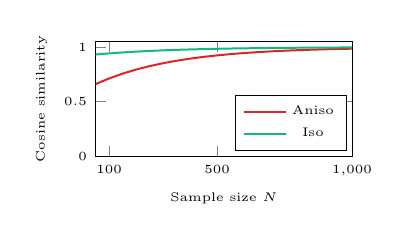
\begin{tikzpicture}[scale=0.9]
\begin{axis}[
  width=5.2cm, height=3.2cm,
  xlabel={\tiny Sample size $N$},
  ylabel={\tiny Cosine similarity},
  ymin=0, ymax=1.05, xmin=50, xmax=1000,
  xtick={100,500,1000}, ytick={0,0.5,1},
  xticklabel style={font=\tiny},
  yticklabel style={font=\tiny},
  legend style={font=\tiny, at={(0.98,0.05)}, anchor=south east},
]
  \addplot[bad, thick, domain=50:1000, samples=20]
    {1 - 0.4*exp(-x/300)};
  \addplot[good, thick, domain=50:1000, samples=20]
    {1 - 0.08*exp(-x/300)};
  \legend{Aniso, Iso}
\end{axis}
\end{tikzpicture}

\column{0.48\textwidth}
\begin{alertblock}{Lemma 3.2 --- Aniso Amplifies Variance}
\small
\[
\text{tr}\!\left(\text{Var}(\hat\beta_\text{aniso})\right) >
\text{tr}\!\left(\text{Var}(\hat\beta_\text{iso})\right)
\]
\end{alertblock}
\vspace{6pt}
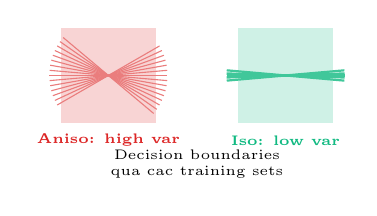
\begin{tikzpicture}[scale=0.75]
  % Anisotropic: many scattered lines
  \begin{scope}
    \filldraw[bad!20] (-0.8,-0.8) rectangle (0.8,0.8);
    \foreach \angle in {-40,-35,-30,-25,-20,-15,-10,-5,0,5,10,15,20,25,30}
      \draw[bad!60, thin]
        ({-1*cos(\angle)},{-1*sin(\angle)}) --
        ({1*cos(\angle)},{1*sin(\angle)});
    \node[bad, font=\tiny\bfseries] at (0,-1.1) {Aniso: high var};
  \end{scope}
  % Isotropic: tight lines
  \begin{scope}[shift={(3,0)}]
    \filldraw[good!20] (-0.8,-0.8) rectangle (0.8,0.8);
    \foreach \angle in {-5,-2,0,2,5}
      \draw[good!80, thick]
        ({-1*cos(\angle)},{-1*sin(\angle)}) --
        ({1*cos(\angle)},{1*sin(\angle)});
    \node[good, font=\tiny\bfseries] at (0,-1.1) {Iso: low var};
  \end{scope}
  \node[font=\tiny, align=center] at (1.5,-1.5)
    {Decision boundaries\\qua cac training sets};
\end{tikzpicture}
\end{columns}
\takeaway{Aniso = chenh + bien dong $\Rightarrow$ Iso thang ca Bias lan Variance}
\end{frame}

% ============================================================
%  SLIDE 10 — Theorem: Nonlinear probe
% ============================================================
\begin{frame}{Chung Minh 2: Iso Gaussian Toi Uu Cho kNN Va Kernel}
\begin{columns}[c]
\column{0.50\textwidth}
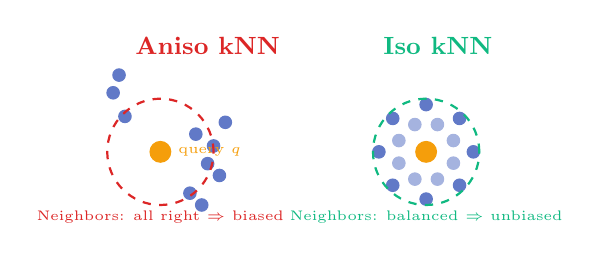
\begin{tikzpicture}[scale=0.75]
  % Anisotropic kNN
  \begin{scope}
    \node[font=\small\bfseries\color{bad}] at (1.8,3.0) {Aniso kNN};
    % Data points clustered to right
    \foreach \x/\y in {1.5/0.5, 1.8/1.0, 1.6/1.5, 2.0/0.8,
                        1.9/1.3, 1.7/0.3, 2.1/1.7}
      \filldraw[primary!70] (\x,\y) circle (3pt);
    \foreach \x/\y in {0.2/2.2, 0.4/1.8, 0.3/2.5}
      \filldraw[primary!70] (\x,\y) circle (3pt);
    % Query
    \filldraw[accent] (1.0,1.2) circle (5pt)
      node[right=3pt, font=\tiny] {query $q$};
    % Neighborhood circle
    \draw[bad, dashed, thick] (1.0,1.2) circle (0.9cm);
    \node[bad, font=\tiny] at (1.0,0.1) {Neighbors: all right $\Rightarrow$ biased};
  \end{scope}
  % Isotropic kNN
  \begin{scope}[shift={(4.5,0)}]
    \node[font=\small\bfseries\color{good}] at (1.2,3.0) {Iso kNN};
    % Points distributed evenly
    \foreach \a in {0,45,...,315}
      \filldraw[primary!70] ({1.0+0.8*cos(\a)},{1.2+0.8*sin(\a)}) circle (3pt);
    \foreach \a in {22.5,67.5,...,337.5}
      \filldraw[primary!40] ({1.0+0.5*cos(\a)},{1.2+0.5*sin(\a)}) circle (3pt);
    \filldraw[accent] (1.0,1.2) circle (5pt);
    \draw[good, dashed, thick] (1.0,1.2) circle (0.9cm);
    \node[good, font=\tiny] at (1.0,0.1) {Neighbors: balanced $\Rightarrow$ unbiased};
  \end{scope}
\end{tikzpicture}

\column{0.47\textwidth}
\begin{block}{Theorem 3.3 --- Iso Gaussian Optimality}
\small Voi constraint $\text{Tr}(\text{Cov}(\mathbf{Z})) = \kappa$:
\[
\text{ISB}_{k\text{-NN}} = \frac{r_0^4}{(K+2)^2}\tau_g^2 J(p) + O(r_0^4)
\]
\textbf{Isotropic Gaussian la nghiem DUY NHAT} minimize ISB cho ca kNN va kernel regression.
\end{block}
\vspace{8pt}
\begin{exampleblock}{Tai sao duy nhat?}
\small Fisher information $J(p)$ duoc minimize khi va chi khi $p = \mathcal{N}(0,I)$\\
$\Rightarrow$ Khong co distribution nao khac dat duoc
\end{exampleblock}
\end{columns}
\takeaway{Optimal cho linear AND nonlinear $\Rightarrow$ Universal optimum}
\end{frame}

% ============================================================
%  SLIDE 11 — Geometric Intuition
% ============================================================
\begin{frame}{Geometric Intuition: Hinh Cau La Toi Uu}
\begin{columns}[c]
\column{0.48\textwidth}
\begin{center}
\textbf{\bad{Anisotropic}} --- khoang cach meo
\end{center}
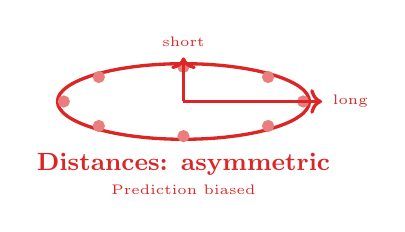
\begin{tikzpicture}[scale=0.8]
  \draw[bad, very thick] (0,0) ellipse (2.0cm and 0.6cm);
  \foreach \a in {0,45,90,135,180,225,270,315}
    \filldraw[bad!60] ({1.9*cos(\a)},{0.55*sin(\a)}) circle (2.5pt);
  % Unequal arrows
  \draw[->, bad, very thick] (0,0) -- (2.2,0) node[right,font=\tiny] {long};
  \draw[->, bad, very thick] (0,0) -- (0,0.7) node[above,font=\tiny] {short};
  \node[bad, font=\small\bfseries] at (0,-1.0) {Distances: asymmetric};
  \node[bad, font=\tiny] at (0,-1.4) {Prediction biased};
\end{tikzpicture}

\column{0.48\textwidth}
\begin{center}
\textbf{\good{Isotropic Gaussian}} --- khoang cach deu
\end{center}
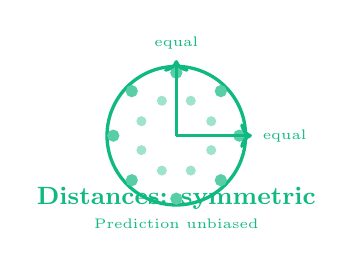
\begin{tikzpicture}[scale=0.8]
  \draw[good, very thick] (0,0) circle (1.1cm);
  \foreach \a in {0,45,90,135,180,225,270,315}
    \filldraw[good!70] ({1.0*cos(\a)},{1.0*sin(\a)}) circle (2.5pt);
  \foreach \a in {22.5,67.5,112.5,157.5,202.5,247.5,292.5,337.5}
    \filldraw[good!40] ({0.6*cos(\a)},{0.6*sin(\a)}) circle (2pt);
  % Equal arrows
  \draw[->, good, very thick] (0,0) -- (1.2,0) node[right,font=\tiny] {equal};
  \draw[->, good, very thick] (0,0) -- (0,1.2) node[above,font=\tiny] {equal};
  \node[good, font=\small\bfseries] at (0,-1.0) {Distances: symmetric};
  \node[good, font=\tiny] at (0,-1.4) {Prediction unbiased};
\end{tikzpicture}
\end{columns}
\vspace{6pt}
\begin{exampleblock}{Analogy}
\small Giong ban do Mercator vs ban do dang dien: Mercator keo dai o vung cuc $\to$ sai so khoang cach.\\
$\mathcal{N}(0,I)$ = ``ban do phang'' cua embedding space --- moi huong nhu nhau.
\end{exampleblock}
\takeaway{$\mathcal{N}(0,I)$: geometry doi xung $\Rightarrow$ moi downstream task deu duoc xu ly cong bang}
\end{frame}

% ============================================================
%  SLIDE 12 — Summary theory + transition
% ============================================================
\begin{frame}{Ket Luan Ly Thuyet: Design Principle}
\begin{center}
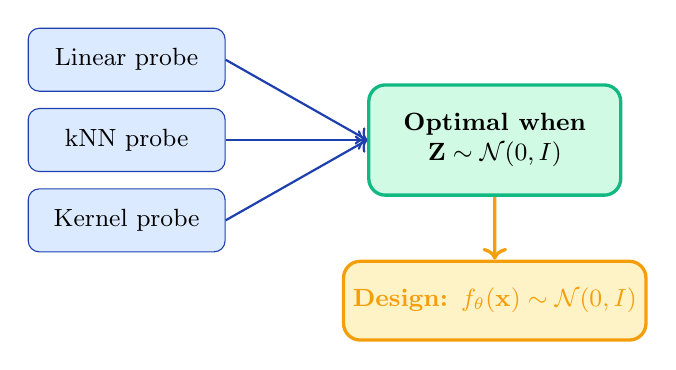
\begin{tikzpicture}[scale=0.85]
  % Three probe types
  \node[draw=primary, fill=lightblue, rounded corners=4pt,
        minimum width=2.5cm, minimum height=0.8cm, font=\small] (lp)
        at (0,2) {Linear probe};
  \node[draw=primary, fill=lightblue, rounded corners=4pt,
        minimum width=2.5cm, minimum height=0.8cm, font=\small] (knn)
        at (0,0.8) {kNN probe};
  \node[draw=primary, fill=lightblue, rounded corners=4pt,
        minimum width=2.5cm, minimum height=0.8cm, font=\small] (ker)
        at (0,-0.4) {Kernel probe};
  % Result
  \node[draw=good, very thick, fill=lightgreen, rounded corners=6pt,
        minimum width=3.2cm, minimum height=1.4cm, align=center,
        font=\small\bfseries] (opt) at (5.5,0.8)
        {Optimal when\\$\mathbf{Z} \sim \mathcal{N}(0,I)$};
  % Arrows
  \draw[->, thick, primary] (lp.east) -- (opt.west);
  \draw[->, thick, primary] (knn.east) -- (opt.west);
  \draw[->, thick, primary] (ker.east) -- (opt.west);
  % Implication
  \node[draw=accent, very thick, fill=lightyellow, rounded corners=6pt,
        minimum width=3.8cm, minimum height=1.0cm, align=center,
        font=\small\bfseries\color{accent}] (des) at (5.5,-1.6)
        {Design: $f_\theta(\mathbf{x}) \sim \mathcal{N}(0,I)$};
  \draw[->, very thick, accent] (opt) -- (des);
\end{tikzpicture}
\end{center}
\vspace{4pt}
\begin{center}
\begin{tabular}{lcc}
\toprule
& \textbf{Prior SSL} & \textbf{LeJEPA} \\
\midrule
Ly do chon distribution & ``It works'' & \good{Proven optimal} \\
Guarantee & \bad{Khong co} & \good{Unique minimizer} \\
Ca linear + nonlinear & \bad{Chua ro} & \good{Ca hai} \\
\bottomrule
\end{tabular}
\end{center}
\takeaway{Lan dau tien: biet CHINH XAC embeddings nen phan phoi the nao}
\end{frame}

% ============================================================
%  SLIDE 13 — Challenge: Testing in high-dim
% ============================================================
\begin{frame}{Thach Thuc: Test Distribution Trong High-Dim}
\begin{columns}[c]
\column{0.55\textwidth}
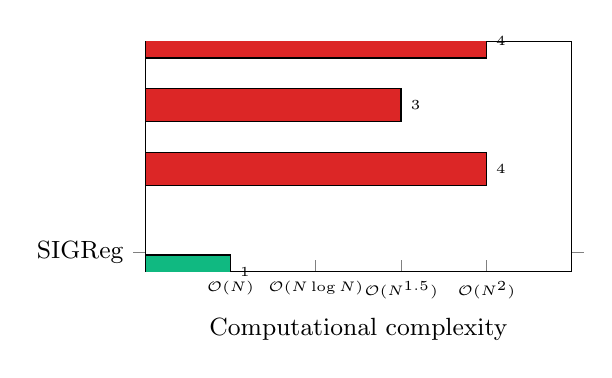
\begin{tikzpicture}
\begin{axis}[
  xbar, width=7cm, height=4.5cm,
  xlabel={\small Computational complexity},
  symbolic y coords={SIGReg, Direct test, KL div., MMD},
  ytick=data,
  yticklabel style={font=\small},
  xticklabel style={font=\tiny},
  xmin=0, xmax=5,
  xtick={1,2,3,4},
  xticklabels={$\mathcal{O}(N)$, $\mathcal{O}(N\log N)$,
               $\mathcal{O}(N^{1.5})$, $\mathcal{O}(N^2)$},
  nodes near coords,
  nodes near coords style={font=\tiny},
]
  \addplot[fill=good, bar width=12pt] coordinates
    {(1,SIGReg)};
  \addplot[fill=bad, bar width=12pt] coordinates
    {(4,MMD)(3,{KL div.})(4,{Direct test})};
\end{axis}
\end{tikzpicture}

\column{0.42\textwidth}
\textbf{3 yeu cau can co:}
\vspace{4pt}

\begin{tabular}{lcc}
& SIGReg & Others \\
\midrule
Differentiable & \good{\checkmark} & \bad{\ding{55}} \\
$\mathcal{O}(N)$ & \good{\checkmark} & \bad{\ding{55}} \\
Provably correct & \good{\checkmark} & partial \\
DDP-friendly & \good{\checkmark} & \bad{\ding{55}} \\
\end{tabular}
\vspace{8pt}

\begin{alertblock}{Curse of Dimensionality}
\small Moi multivariate normality test chuan (Henze-Zirkler, BHEP, Mardia): $\mathcal{O}(N^2)$ hoac te hon.
$\Rightarrow$ Can strategy khac!
\end{alertblock}
\end{columns}
\takeaway{Existing tools khong scale $\Rightarrow$ can sketching strategy}
\end{frame}

% ============================================================
%  SLIDE 14 — 1D Slicing (Cramer-Wold)
% ============================================================
\begin{frame}{Giai Phap: Sketch Qua Random 1D Projections}
\begin{columns}[c]
\column{0.50\textwidth}
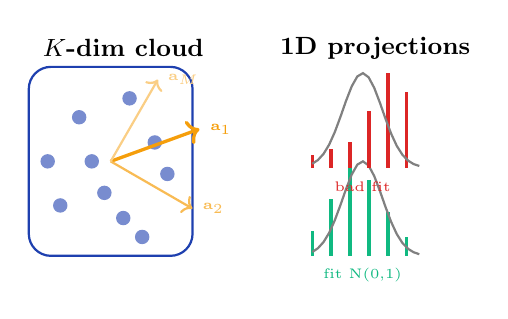
\begin{tikzpicture}[scale=0.8]
  % 2D cloud (representing K-dim)
  \begin{scope}
    \node[font=\small\bfseries] at (1.5,3.3) {$K$-dim cloud};
    \foreach \x/\y in {0.5/0.8, 1.0/1.5, 1.5/0.6, 2.0/1.8,
                        0.8/2.2, 1.8/0.3, 1.2/1.0, 2.2/1.3,
                        0.3/1.5, 1.6/2.5}
      \filldraw[primary!60] (\x,\y) circle (3pt);
    \draw[primary, thick, rounded corners=8pt]
      (0,0) rectangle (2.6,3.0);
  \end{scope}
  % Direction arrows
  \draw[->, accent, very thick, rotate around={20:(1.3,1.5)}]
    (1.3,1.5) -- (2.8,1.5) node[right, accent, font=\tiny] {$\mathbf{a}_1$};
  \draw[->, accent!70, thick, rotate around={-30:(1.3,1.5)}]
    (1.3,1.5) -- (2.8,1.5) node[right, accent!70, font=\tiny] {$\mathbf{a}_2$};
  \draw[->, accent!50, thick, rotate around={60:(1.3,1.5)}]
    (1.3,1.5) -- (2.8,1.5) node[right, accent!50, font=\tiny] {$\mathbf{a}_M$};
  % 1D histograms (right side)
  \begin{scope}[shift={(4.5,0)}]
    \node[font=\small\bfseries] at (1.0,3.3) {1D projections};
    % Histogram 1 (good fit)
    \foreach \h/\x in {0.4/0, 0.9/0.3, 1.4/0.6, 1.2/0.9, 0.7/1.2, 0.3/1.5}
      \draw[good, very thick] (\x,0) -- (\x,\h);
    \draw[black!50, thick, domain=0:1.7, samples=20]
      plot (\x, {1.5*exp(-(\x-0.8)^2/0.2)});
    \node[good, font=\tiny] at (0.8,-0.3) {fit N(0,1)};
    % Histogram 2 (bad fit)
    \begin{scope}[shift={(0,1.4)}]
      \foreach \h/\x in {0.2/0, 0.3/0.3, 0.4/0.6, 0.9/0.9, 1.5/1.2, 1.2/1.5}
        \draw[bad, very thick] (\x,0) -- (\x,\h);
      \draw[black!50, thick, domain=0:1.7, samples=20]
        plot (\x, {1.5*exp(-(\x-0.8)^2/0.2)});
      \node[bad, font=\tiny] at (0.8,-0.3) {bad fit};
    \end{scope}
  \end{scope}
\end{tikzpicture}

\column{0.47\textwidth}
\begin{block}{Hyperspherical Cramer-Wold (Lemma 4.1)}
\small
\[
X \stackrel{d}{=} Y \iff
\langle \mathbf{u}, X\rangle \stackrel{d}{=} \langle \mathbf{u}, Y\rangle
\quad \forall\, \mathbf{u} \in \mathbb{S}^{K-1}
\]
\end{block}
\vspace{6pt}
\textbf{Practical version:}\\
Khong can ALL directions --- sample $M$ ngau nhien + reuse qua training steps.
\vspace{6pt}

\begin{exampleblock}{Theorem 4.2 (Consistency)}
\small Voi $M$ random directions, test van consistent (level + power) khi $M \to \infty$ cung training.
\end{exampleblock}
\end{columns}
\takeaway{Bai toan $K$-chieu $\to$ $M$ bai toan 1-chieu doc lap}
\end{frame}

% ============================================================
%  SLIDE 15 — Comparing 3 families of 1D tests
% ============================================================
\begin{frame}{Chon Test 1D Nao? So Sanh 3 Ho}
\begin{center}
\begin{tabular}{p{2.2cm}p{2.5cm}p{2.0cm}p{3.5cm}}
\toprule
\textbf{Ho} & \textbf{Test tiêu bieu} & \textbf{Differentiable} & \textbf{Van de} \\
\midrule
\cellcolor{lightred}\textbf{Moment-based}
  & Jarque-Bera, EJB
  & \cellcolor{lightred}\bad{\ding{55}} Unstable
  & Gradient $\propto x^k$: explode\\
  & & & $K$ moments finite $\not\Rightarrow P=Q$ \\[4pt]
\cellcolor{lightred}\textbf{CDF-based}
  & Cramer-von Mises, Anderson-Darling
  & \cellcolor{lightred}\bad{\ding{55}} Non-diff
  & Can sort: $\mathcal{O}(N\log N)$, non-parallel\\
  & & & Soft sort: them hyperparameters \\[4pt]
\cellcolor{lightgreen}\textbf{CF-based} $\bigstar$
  & \textbf{Epps-Pulley}
  & \cellcolor{lightgreen}\good{\checkmark} Bounded
  & \good{Khong co van de} \\
  & & & \good{$|\partial EP/\partial z| \leq 4\sigma^2/N$} \\
\bottomrule
\end{tabular}
\end{center}
\vspace{6pt}
\begin{alertblock}{Theorem 4.3 --- Moment Insufficiency}
\small Minimize $\sum_{k=1}^K c_k(m_k(P_\theta) - m_k(Q))^2$ voi finite $K$ \textbf{khong} imply $P_\theta = Q$
$\Rightarrow$ Shortcut solutions ton tai!
\end{alertblock}
\takeaway{Epps-Pulley = sweet spot duy nhat: differentiable + O(N) + bounded gradient}
\end{frame}

% ============================================================
%  SLIDE 16 — Epps-Pulley test
% ============================================================
\begin{frame}{Epps-Pulley Test: Stable, Scalable, Provable}
\begin{columns}[c]
\column{0.50\textwidth}
\begin{block}{Epps-Pulley Statistic}
\[
EP = N\!\int_{-\infty}^{\infty}
\underbrace{|\hat\phi_X(t) - \phi(t)|^2}_{\text{ECF vs target CF}}
\underbrace{e^{-t^2/2}}_{\text{Gauss window}}
dt
\]
\[
\hat\phi_X(t) = \tfrac{1}{N}\textstyle\sum_j e^{itX_j}, \quad
\phi(t) = e^{-t^2/2}
\]
\end{block}
\vspace{6pt}
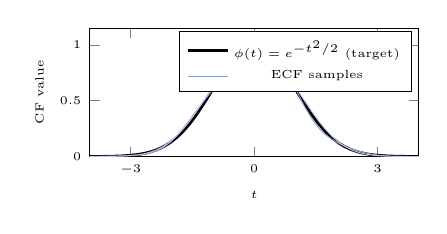
\begin{tikzpicture}[scale=0.85]
\begin{axis}[
  width=6.5cm, height=3.5cm,
  xlabel={\tiny $t$}, ylabel={\tiny CF value},
  xmin=-4, xmax=4, ymin=0, ymax=1.15,
  xtick={-3,0,3}, ytick={0,0.5,1},
  xticklabel style={font=\tiny},
  yticklabel style={font=\tiny},
  legend style={font=\tiny, at={(0.98,0.98)}, anchor=north east},
]
  % Theoretical CF
  \addplot[black, very thick, domain=-4:4, samples=50]
    {exp(-x^2/2)};
  % Empirical CFs (simulate noise)
  \addplot[primary!50, thin, domain=-4:4, samples=50]
    {exp(-x^2/2) + 0.08*sin(3*deg(x))*exp(-x^2/3)};
  \addplot[primary!30, thin, domain=-4:4, samples=50]
    {exp(-x^2/2) - 0.06*cos(2*deg(x))*exp(-x^2/3)};
  \legend{$\phi(t)=e^{-t^2/2}$ (target), ECF samples}
\end{axis}
\end{tikzpicture}

\column{0.47\textwidth}
\begin{alertblock}{Theorem 4.5 --- Bounded Gradient}
\[
\left|\frac{\partial EP}{\partial z_i}\right| \leq \frac{4\sigma^2}{N}
\]
\[
\left|\frac{\partial^2 EP}{\partial z_i^2}\right| \leq \frac{C\sqrt{\pi}\sigma^3}{2N}
\]
\small Bat ke distribution input --- LUON bounded
\end{alertblock}
\vspace{6pt}
\textbf{3 ly do chon EP:}
\begin{itemize}\small
  \item[\good{\checkmark}] ECF = average of $e^{itX_j}$: differentiable, bounded trong $[-1,1]$
  \item[\good{\checkmark}] $\mathcal{O}(N)$: sum, khong sort
  \item[\good{\checkmark}] \texttt{all\_reduce}: DDP-friendly
\end{itemize}
\end{columns}
\takeaway{ECF bounded $\Rightarrow$ gradient khong bao gio explode, bat ke distribution}
\end{frame}

% ============================================================
%  SLIDE 17 — SIGReg Definition
% ============================================================
\begin{frame}{SIGReg: Cong Thuc Hoan Chinh}
\begin{columns}[c]
\column{0.50\textwidth}
\begin{block}{Definition: SIGReg}
\[
\text{SIGReg}(\mathcal{A},\{f_\theta(\mathbf{x}_n)\}) =
\frac{1}{|\mathcal{A}|}\sum_{\mathbf{a}\in\mathcal{A}}
EP\!\left(\{\mathbf{a}^\top f_\theta(\mathbf{x}_n)\}_{n=1}^N\right)
\]
\end{block}
\vspace{6pt}
\begin{lstlisting}[language=Python, caption={}]
def SIGReg(x, step, M=1024):
  g = torch.Generator(device=x.device)
  g.manual_seed(step)        # sync GPUs
  A = torch.randn(x.size(1), M, generator=g)
  A /= A.norm(p=2, dim=0)    # unit vectors
  t = torch.linspace(0, 3, 17)
  phi = torch.exp(-0.5*t**2) # N(0,1) CF
  x_t = (x @ A).unsqueeze(-1) * t  # (N,M,T)
  err = (x_t.cos().mean(0)-phi)**2 \
      +  x_t.sin().mean(0)**2
  return (err @ weights).mean() * N
\end{lstlisting}

\column{0.47\textwidth}
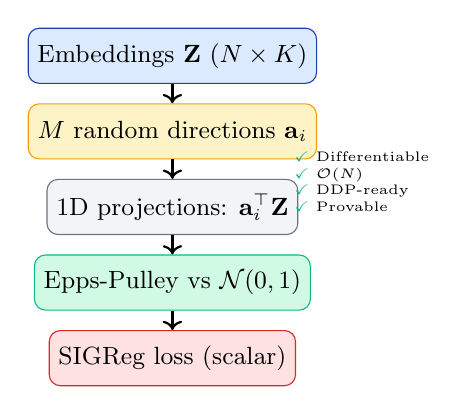
\begin{tikzpicture}[scale=0.8]
  % Pipeline
  \node[draw=primary, fill=lightblue, rounded corners=4pt,
        minimum width=3cm, minimum height=0.7cm] (emb) at (0,4)
        {\small Embeddings $\mathbf{Z}$ ($N\times K$)};
  % Directions
  \node[draw=accent, fill=lightyellow, rounded corners=4pt,
        minimum width=3cm, minimum height=0.7cm] (dir) at (0,2.8)
        {\small $M$ random directions $\mathbf{a}_i$};
  % Projections
  \node[draw=neutral, fill=lightgray, rounded corners=4pt,
        minimum width=3cm, minimum height=0.7cm] (proj) at (0,1.6)
        {\small 1D projections: $\mathbf{a}_i^\top \mathbf{Z}$};
  % EP test
  \node[draw=good, fill=lightgreen, rounded corners=4pt,
        minimum width=3cm, minimum height=0.7cm] (ep) at (0,0.4)
        {\small Epps-Pulley vs $\mathcal{N}(0,1)$};
  % Output
  \node[draw=bad, fill=lightred, rounded corners=4pt,
        minimum width=3cm, minimum height=0.7cm] (out) at (0,-0.8)
        {\small SIGReg loss (scalar)};
  % Arrows
  \foreach \a/\b in {emb/dir, dir/proj, proj/ep, ep/out}
    \draw[->, thick] (\a) -- (\b);
  % Properties
  \node[font=\tiny, align=left] at (3.0,2.0)
    {\good{\checkmark} Differentiable\\
     \good{\checkmark} $\mathcal{O}(N)$\\
     \good{\checkmark} DDP-ready\\
     \good{\checkmark} Provable};
\end{tikzpicture}
\end{columns}
\takeaway{50 dong code PyTorch --- chay tren bat ky GPU/TPU nao}
\end{frame}

% ============================================================
%  SLIDE 18 — Curse of Dimensionality
% ============================================================
\begin{frame}{SIGReg Thoat Khoi Curse of Dimensionality}
\begin{columns}[t]
\column{0.48\textwidth}
\textbf{Fixed vs Resampled directions:}
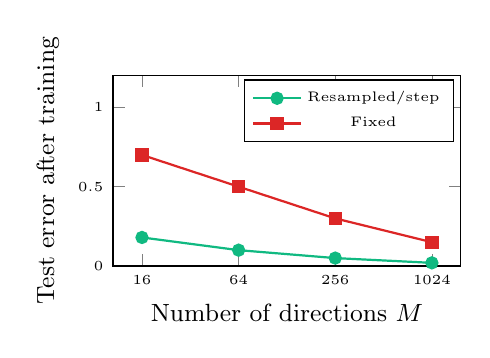
\begin{tikzpicture}
\begin{axis}[
  width=6cm, height=4cm,
  xlabel={\small Number of directions $M$},
  ylabel={\small Test error after training},
  xmode=log, log ticks with fixed point,
  xtick={16,64,256,1024},
  xticklabels={16,64,256,1024},
  xticklabel style={font=\tiny},
  yticklabel style={font=\tiny},
  ymin=0, ymax=1.2,
  legend style={font=\tiny, at={(0.98,0.98)}, anchor=north east},
]
  \addplot[good, thick, mark=*, mark size=2pt]
    coordinates {(16,0.18)(64,0.10)(256,0.05)(1024,0.02)};
  \addplot[bad, thick, mark=square*, mark size=2pt]
    coordinates {(16,0.70)(64,0.50)(256,0.30)(1024,0.15)};
  \legend{Resampled/step, Fixed}
\end{axis}
\end{tikzpicture}

\column{0.48\textwidth}
\textbf{Error bound (Theorem 4.7):}
\begin{block}{}
\small
\[
\mathbb{E}_\mathbf{a}[\cdots] \leq
C(K,\alpha)\cdot |\mathcal{A}|^{-\frac{2\alpha}{K-1}}
\cdot \|\cdot\|_{H^\alpha}^2
\]
Khi $\alpha$ lon: $|\mathcal{A}| = \mathcal{O}(K)$ du de $\epsilon$-approximation
\end{block}
\vspace{4pt}
\textbf{2 ly do thoat curse:}
\begin{enumerate}\small
  \item \textbf{Smoothness:} DNN naturally smooth (BN, dropout, WD) $\to$ $\alpha$ lon $\to$ $M$ nho du
  \item \textbf{SGD resampling:} Qua $T$ steps, tong directions = $M\times T \to \infty$
\end{enumerate}
\vspace{4pt}
\begin{exampleblock}{}
\small $M=16$ resampled $\approx$ $M=1000$ fixed\\
$\Rightarrow$ Overhead nho nhung hieu qua lon
\end{exampleblock}
\end{columns}
\takeaway{Smoothness + resampling: $M=16$ du du $K=2048$}
\end{frame}

% ============================================================
%  SLIDE 19 — LeJEPA Loss
% ============================================================
\begin{frame}{LeJEPA Loss: Ket Hop 2 Thanh Phan}
\small
\[
\mathcal{L}_\text{LeJEPA} =
\underbrace{(1-\lambda)\cdot
  \frac{1}{B}\sum_{n=1}^B
  \frac{1}{V}\sum_{v=1}^V\|\bm{\mu}_n - \mathbf{z}_{n,v}\|_2^2
}_{\text{Invariance: cac views phai agree}} +
\underbrace{
  \frac{\lambda}{V}\sum_{v=1}^V \text{SIGReg}(\{\mathbf{z}_{n,v}\}_{n=1}^B)
}_{\text{SIGReg: push ve }\mathcal{N}(0,I)}
\]
\vspace{4pt}
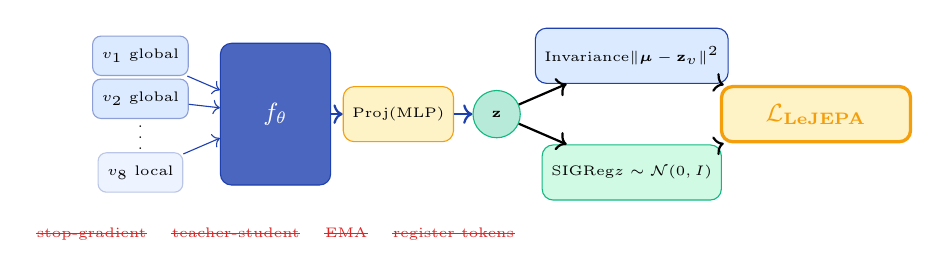
\begin{tikzpicture}[scale=0.78, node distance=0.5cm]
  % Views
  \node[draw=primary!50, fill=lightblue, rounded corners=3pt,
        minimum width=1.0cm, minimum height=0.5cm, font=\tiny] (v1) at (0,1.6) {$v_1$ global};
  \node[draw=primary!50, fill=lightblue, rounded corners=3pt,
        minimum width=1.0cm, minimum height=0.5cm, font=\tiny] (v2) at (0,0.9) {$v_2$ global};
  \node[font=\tiny] at (0,0.4) {$\vdots$};
  \node[draw=primary!30, fill=lightblue!50, rounded corners=3pt,
        minimum width=1.0cm, minimum height=0.5cm, font=\tiny] (v8) at (0,-0.3) {$v_8$ local};
  % Encoder
  \node[draw=primary, fill=primary!80, text=white, rounded corners=4pt,
        minimum width=1.4cm, minimum height=1.8cm, font=\small\bfseries] (enc) at (2.2,0.65)
        {$f_\theta$};
  % Proj
  \node[draw=accent, fill=lightyellow, rounded corners=4pt,
        minimum width=1.4cm, minimum height=0.7cm, font=\tiny] (proj) at (4.2,0.65)
        {Proj\\(MLP)};
  % z
  \node[circle, draw=good, fill=good!30, minimum size=0.6cm, font=\tiny] (z) at (5.8,0.65)
        {$\mathbf{z}$};
  % Two losses
  \node[draw=primary, fill=lightblue, rounded corners=4pt,
        minimum width=2.2cm, minimum height=0.7cm, font=\tiny] (inv) at (8.0,1.6)
        {Invariance\\$\|\bm\mu - \mathbf{z}_v\|^2$};
  \node[draw=good, fill=lightgreen, rounded corners=4pt,
        minimum width=2.2cm, minimum height=0.7cm, font=\tiny] (sig) at (8.0,-0.3)
        {SIGReg\\$z\sim\mathcal{N}(0,I)$};
  % Total
  \node[draw=accent, very thick, fill=lightyellow, rounded corners=4pt,
        minimum width=2.4cm, minimum height=0.7cm, font=\small\bfseries\color{accent}] (tot) at (11.0,0.65)
        {$\mathcal{L}_\text{LeJEPA}$};
  % Arrows
  \foreach \s in {v1,v2,v8}
    \draw[->, thin, primary] (\s) -- (enc);
  \draw[->, thick, primary] (enc) -- (proj);
  \draw[->, thick, primary] (proj) -- (z);
  \draw[->, thick] (z) -- (inv);
  \draw[->, thick] (z) -- (sig);
  \draw[->, thick] (inv) -- (tot);
  \draw[->, thick] (sig) -- (tot);
  % Removed items (strikethrough)
  \node[bad, font=\tiny, align=left] at (2.2,-1.3)
    {\sout{stop-gradient} \quad \sout{teacher-student} \quad
     \sout{EMA} \quad \sout{register tokens}};
\end{tikzpicture}
\takeaway{1 loss $\cdot$ 1 hyperparameter $\lambda$ $\cdot$ 0 heuristic}
\end{frame}

% ============================================================
%  SLIDE 20 — LeJEPA vs Prior Work
% ============================================================
\begin{frame}{LeJEPA vs DINO / I-JEPA: Head-to-Head}
\begin{center}
\begin{tabular}{lccc}
\toprule
\textbf{Tieu chi} & \textbf{DINO} & \textbf{I-JEPA} & \textbf{LeJEPA} \\
\midrule
Anti-collapse
  & \cellcolor{lightred}EMA+stop-grad
  & \cellcolor{lightred}Stop-grad+mask
  & \cellcolor{lightgreen}\good{\textbf{Theorem}} \\[3pt]
\# Hyperparameters
  & \cellcolor{lightred}$\geq$7
  & \cellcolor{lightred}$\geq$5
  & \cellcolor{lightgreen}\good{\textbf{1 ($\lambda$)}} \\[3pt]
Complexity
  & $\mathcal{O}(N)$
  & $\mathcal{O}(N)$
  & \cellcolor{lightgreen}\good{$\mathcal{O}(N)$} \\[3pt]
Architecture
  & \cellcolor{lightred}ViT only
  & \cellcolor{lightred}ViT preferred
  & \cellcolor{lightgreen}\good{\textbf{Any (60+)}} \\[3pt]
Loss informativeness
  & \cellcolor{lightred}$\sim$20\% corr.
  & \cellcolor{lightred}$\sim$30\% corr.
  & \cellcolor{lightgreen}\good{\textbf{94\% Spearman}} \\[3pt]
Theory foundation
  & \cellcolor{lightred}Post-hoc
  & \cellcolor{lightred}Post-hoc
  & \cellcolor{lightgreen}\good{\textbf{First-principles}} \\[3pt]
Core code (lines)
  & \cellcolor{lightred}1000+
  & \cellcolor{lightred}500+
  & \cellcolor{lightgreen}\good{\textbf{$\approx$50}} \\
\bottomrule
\end{tabular}
\end{center}
\takeaway{Don gian hon + ly thuyet chac hon + work tren moi kien truc}
\end{frame}

% ============================================================
%  SLIDE 21 — Lambda tradeoff
% ============================================================
\begin{frame}{$\lambda$: Nut Duy Nhat Can Chinh}
\begin{columns}[c]
\column{0.50\textwidth}
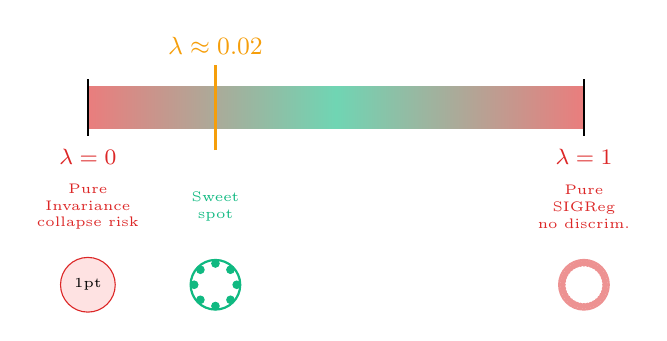
\begin{tikzpicture}[scale=0.9]
  % Spectrum bar
  \shade[left color=bad!60, right color=bad!60, middle color=good!60]
    (0,0.6) rectangle (7,1.2);
  % Tick marks
  \draw[thick] (0,0.5) -- (0,1.3);
  \draw[thick] (7,0.5) -- (7,1.3);
  \draw[very thick, accent] (1.8,0.3) -- (1.8,1.5)
    node[above, accent, font=\small\bfseries] {$\lambda\approx0.02$};
  % Labels
  \node[bad, font=\footnotesize\bfseries] at (0.0, 0.2) {$\lambda=0$};
  \node[bad, font=\footnotesize\bfseries] at (7.0, 0.2) {$\lambda=1$};
  \node[bad, font=\tiny, align=center] at (0.0,-0.5)
    {Pure\\Invariance\\collapse risk};
  \node[bad, font=\tiny, align=center] at (7.0,-0.5)
    {Pure\\SIGReg\\no discrim.};
  \node[good, font=\tiny, align=center] at (1.8,-0.5)
    {Sweet\\spot};
  % Embedding cloud sketches
  \node[draw=bad, fill=lightred, minimum size=0.6cm,
        circle, font=\tiny] at (0,-1.6) {1pt};
  \draw[good, thick] (1.8,-1.6) circle (0.35cm);
  \foreach \a in {0,45,...,315}
    \filldraw[good] ({1.8+0.3*cos(\a)},{-1.6+0.3*sin(\a)}) circle (1.5pt);
  \draw[bad!50, thick] (7,-1.6) circle (0.35cm);
  \foreach \a in {0,10,...,350}
    \filldraw[bad!50] ({7+0.3*cos(\a)},{-1.6+0.3*sin(\a)}) circle (1pt);
\end{tikzpicture}

\column{0.47\textwidth}
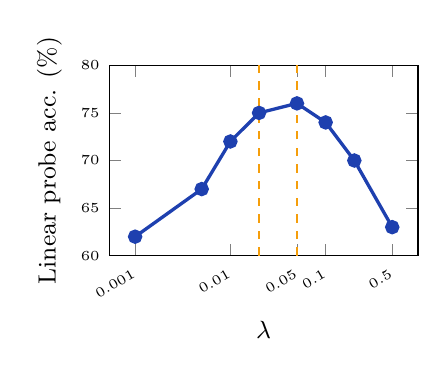
\begin{tikzpicture}
\begin{axis}[
  width=5.5cm, height=4cm,
  xlabel={\small $\lambda$},
  ylabel={\small Linear probe acc. (\%)},
  xmode=log,
  xtick={0.001,0.01,0.05,0.1,0.5},
  xticklabels={0.001,0.01,0.05,0.1,0.5},
  xticklabel style={font=\tiny, rotate=30, anchor=north east},
  yticklabel style={font=\tiny},
  ymin=60, ymax=80,
]
  \addplot[primary, very thick, mark=*, mark size=2pt]
    coordinates{(0.001,62)(0.005,67)(0.01,72)(0.02,75)(0.05,76)
                (0.1,74)(0.2,70)(0.5,63)};
  \draw[accent, dashed, thick] (axis cs:0.02,60) -- (axis cs:0.02,80)
    node[above, accent, font=\tiny] {rec.};
  \draw[accent, dashed, thick] (axis cs:0.05,60) -- (axis cs:0.05,80)
    node[above, accent, font=\tiny] {rec.};
\end{axis}
\end{tikzpicture}
\vspace{4pt}
\begin{block}{Recommended defaults}
\footnotesize
$\lambda=0.05$, $V_g=2$, $V_l=6$,\\
batch $\geq 128$, slices $=1024$
\end{block}
\end{columns}
\takeaway{$\lambda$ robust tren dai rong --- khong can grid search}
\end{frame}

% ============================================================
%  SLIDE 22 — Informative loss
% ============================================================
\begin{frame}{Bonus: Training Loss Du Doan Duoc Downstream Performance}
\begin{columns}[c]
\column{0.50\textwidth}
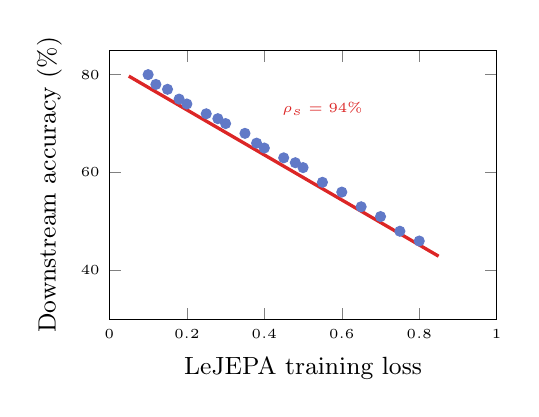
\begin{tikzpicture}
\begin{axis}[
  width=6.5cm, height=5cm,
  xlabel={\small LeJEPA training loss},
  ylabel={\small Downstream accuracy (\%)},
  xmin=0, xmax=1, ymin=30, ymax=85,
  xtick={0,0.2,...,1},
  xticklabel style={font=\tiny},
  yticklabel style={font=\tiny},
  legend style={font=\tiny, at={(0.98,0.05)}, anchor=south east},
]
  % Scatter points (simulated)
  \addplot[only marks, mark=*, mark size=1.8pt, primary!70]
    coordinates{
      (0.1,80)(0.15,77)(0.2,74)(0.25,72)(0.3,70)
      (0.35,68)(0.4,65)(0.45,63)(0.5,61)(0.55,58)
      (0.6,56)(0.65,53)(0.7,51)(0.75,48)(0.8,46)
      (0.12,78)(0.18,75)(0.28,71)(0.38,66)(0.48,62)
    };
  % Regression line
  \addplot[bad, very thick, domain=0.05:0.85]
    {82 - 46*x};
  \node[font=\tiny\bfseries, bad] at (axis cs:0.55,73)
    {$\rho_s = 94\%$};
\end{axis}
\end{tikzpicture}

\column{0.47\textwidth}
\begin{block}{Scaling Law}
\small
\[
C^{(\alpha)} = \rho_s\!\left(
  \frac{\text{train\_loss}}{\lambda^\alpha},
  \text{test\_acc}
\right)
\]
$\alpha=0$: $\rho_s \approx 94\%$\\
$\alpha=0.4$: $\rho_s \approx 99\%$
\end{block}
\vspace{8pt}
\begin{center}
\begin{tabular}{lc}
\toprule
Method & Loss corr. \\
\midrule
DINO & $\sim$20\% \\
I-JEPA & $\sim$30\% \\
\good{\textbf{LeJEPA}} & \good{\textbf{94\%}} \\
\bottomrule
\end{tabular}
\end{center}
\vspace{6pt}
\begin{exampleblock}{Implication}
\small Khong can chay full linear probe de chon model! Dung training loss truc tiep $\to$ tiet kiem 90\% compute.
\end{exampleblock}
\end{columns}
\takeaway{Lan dau tien: SSL co training signal thuc su co nghia}
\end{frame}

% ============================================================
%  SLIDE 23 — VICReg as special case
% ============================================================
\begin{frame}{Ket Noi Voi Prior Work: VICReg La Special Case}
\begin{columns}[c]
\column{0.50\textwidth}
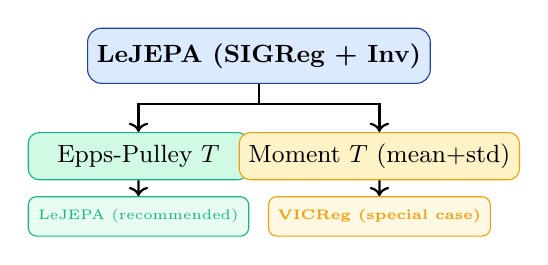
\begin{tikzpicture}[scale=0.85]
  % Root
  \node[draw=primary, fill=lightblue, rounded corners=5pt,
        minimum width=3cm, minimum height=0.7cm, font=\small\bfseries] (root)
        at (0,3) {LeJEPA (SIGReg + Inv)};
  % Branch 1
  \node[draw=good, fill=lightgreen, rounded corners=4pt,
        minimum width=2.8cm, minimum height=0.6cm, font=\small] (b1)
        at (-1.8,1.5) {Epps-Pulley $T$};
  \node[draw=good, fill=lightgreen!50, rounded corners=3pt,
        minimum width=2.8cm, minimum height=0.5cm, font=\tiny] (b1r)
        at (-1.8,0.6) {\good{LeJEPA (recommended)}};
  % Branch 2
  \node[draw=accent, fill=lightyellow, rounded corners=4pt,
        minimum width=2.8cm, minimum height=0.6cm, font=\small] (b2)
        at (1.8,1.5) {Moment $T$ (mean+std)};
  \node[draw=accent, fill=lightyellow!50, rounded corners=3pt,
        minimum width=2.8cm, minimum height=0.5cm, font=\tiny] (b2r)
        at (1.8,0.6) {\hl{VICReg (special case)}};
  % Arrows
  \draw[->, thick] (root.south) -- ++(0,-0.3) -| (b1.north);
  \draw[->, thick] (root.south) -- ++(0,-0.3) -| (b2.north);
  \draw[->, thick] (b1) -- (b1r);
  \draw[->, thick] (b2) -- (b2r);
\end{tikzpicture}

\column{0.47\textwidth}
\begin{block}{VICReg $\subset$ LeJEPA}
\small Khi $T(\mathbf{u}) = \hat\mu(\mathbf{u})^2 + (\hat\sigma(\mathbf{u})^2-1)^2$:
\[
\text{SIGReg} \xrightarrow{M\to\infty} \text{VICReg variance}
\]
SIGReg dam bao:
$\mathbb{E}[\mathbf{Z}]=\mathbf{0}$, $\text{Cov}(\mathbf{Z})\approx I$
\end{block}
\vspace{8pt}
\begin{alertblock}{Tai sao khong dung VICReg test?}
\small \textbf{Theorem 4.3:} Finite moments $\not\Rightarrow P=Q$\\
$\Rightarrow$ Shortcut solutions ton tai\\
VICReg da quan sat thuc te nay!
\end{alertblock}
\vspace{6pt}
\textbf{Ket luan:} VICReg la instance cua LeJEPA voi \textbf{test yeu hon} -- khong guarantee loai bo collapse.
\end{columns}
\takeaway{VICReg = LeJEPA voi test yeu hon --- giai thich tai sao VICReg co shortcut solutions}
\end{frame}

% ============================================================
%  SLIDE 24 — Stability across architectures
% ============================================================
\begin{frame}{LeJEPA: Stable Tren 50+ Architectures}
\begin{columns}[c]
\column{0.55\textwidth}
\begin{tikzpicture}
\begin{axis}[
  xbar, width=7.5cm, height=6cm,
  xlabel={\small Top-1 Acc. (\%) on ImageNet-10},
  symbolic y coords={
    EfficientNet, MobileNet, Swin-T, ConvNeXt-T,
    MaxViT-T, ResNet-50, ViT-S/16, ViT-B/8},
  ytick=data,
  yticklabel style={font=\tiny},
  xticklabel style={font=\tiny},
  xmin=89, xmax=96,
  bar width=8pt,
  nodes near coords, nodes near coords style={font=\tiny},
]
  \addplot[fill=primary!60, bar width=8pt] coordinates {
    (91.5, EfficientNet)(91.8, MobileNet)(92.5, Swin-T)
    (92.8, ConvNeXt-T)(93.2, MaxViT-T)(93.7, ResNet-50)
    (94.3, ViT-S/16)(94.9, ViT-B/8)
  };
\end{axis}
\end{tikzpicture}

\column{0.42\textwidth}
\begin{block}{Key Numbers}
\begin{itemize}\small
  \item \textbf{50} models from \textbf{8} families
  \item Params: 5M $\to$ 700M
  \item Range: 91.5\% $\to$ 95\%
  \item \good{\textbf{Zero collapses}}
\end{itemize}
\end{block}
\vspace{8pt}
\textbf{Ablation (ViT-L/14, IN-1K):}
\begin{center}
\begin{tabular}{lcc}
\toprule
Config & Change & Acc. \\
\midrule
Batch 128$\to$1024 & +2.5\% & stable \\
Slices 512$\to$4096 & +0.7\% & stable \\
Range [-1,1]$\to$[-5,5] & +2.0\% & stable \\
\bottomrule
\end{tabular}
\end{center}
\vspace{4pt}
\begin{exampleblock}{}
\small Khong co architecture nao can dieu chinh dac biet.
\end{exampleblock}
\end{columns}
\takeaway{50 models, zero collapses --- khong can architecture-specific tuning}
\end{frame}

% ============================================================
%  SLIDE 25 — Hyperparameter Stability
% ============================================================
\begin{frame}{Hyperparameter Stability: Bat Ky Config Cung Work}
\begin{columns}[t]
\column{0.48\textwidth}
\textbf{Views vs Lambda (ResNet-50, IN-100):}
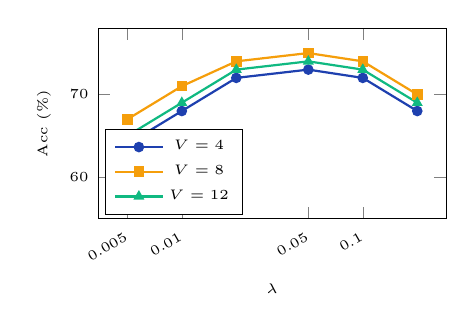
\begin{tikzpicture}
\begin{axis}[
  width=6cm, height=4cm,
  xlabel={\tiny $\lambda$},
  ylabel={\tiny Acc (\%)},
  xmode=log,
  xtick={0.005,0.01,0.05,0.1},
  xticklabels={0.005,0.01,0.05,0.1},
  xticklabel style={font=\tiny, rotate=30, anchor=north east},
  yticklabel style={font=\tiny},
  ymin=55, ymax=78,
  legend style={font=\tiny, at={(0.02,0.02)}, anchor=south west},
]
  \addplot[primary, thick, mark=*,mark size=1.5pt]
    coordinates{(0.005,64)(0.01,68)(0.02,72)(0.05,73)
                (0.1,72)(0.2,68)};
  \addplot[accent, thick, mark=square*,mark size=1.5pt]
    coordinates{(0.005,67)(0.01,71)(0.02,74)(0.05,75)
                (0.1,74)(0.2,70)};
  \addplot[good, thick, mark=triangle*,mark size=1.5pt]
    coordinates{(0.005,65)(0.01,69)(0.02,73)(0.05,74)
                (0.1,73)(0.2,69)};
  \legend{$V=4$,$V=8$,$V=12$}
\end{axis}
\end{tikzpicture}

\column{0.48\textwidth}
\textbf{Batch size \& Projector (ViT-L, IN-1K):}
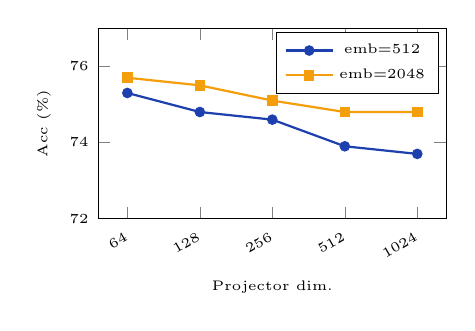
\begin{tikzpicture}
\begin{axis}[
  width=6cm, height=4cm,
  xlabel={\tiny Projector dim.},
  ylabel={\tiny Acc (\%)},
  xmode=log, log ticks with fixed point,
  xtick={64,128,256,512,1024},
  xticklabels={64,128,256,512,1024},
  xticklabel style={font=\tiny, rotate=30, anchor=north east},
  yticklabel style={font=\tiny},
  ymin=72, ymax=77,
  legend style={font=\tiny, at={(0.98,0.98)}, anchor=north east},
]
  \addplot[primary, thick, mark=*,mark size=1.5pt]
    coordinates{(64,75.3)(128,74.8)(256,74.6)(512,73.9)(1024,73.7)};
  \addplot[accent, thick, mark=square*,mark size=1.5pt]
    coordinates{(64,75.7)(128,75.5)(256,75.1)(512,74.8)(1024,74.8)};
  \legend{emb=512, emb=2048}
\end{axis}
\end{tikzpicture}
\vspace{4pt}
\begin{exampleblock}{}
\footnotesize Khong co catastrophic collapse tren bat ky config nao. Batch 128 da competitive.
\end{exampleblock}
\end{columns}
\takeaway{LeJEPA: robust tren bat ky hyperparameter setting hop ly}
\end{frame}

% ============================================================
%  SLIDE 26 — Scale: ViT-H results
% ============================================================
\begin{frame}{LeJEPA Scale: SOTA Voi It Compute Hon}
\begin{columns}[c]
\column{0.50\textwidth}
\textbf{Few-shot transfer (IN-1K pretrain):}
\begin{center}
\begin{tabular}{lrrr}
\toprule
Method & Params & Ep & Avg \\
\midrule
I-JEPA ViT-H & 632M & 300 & 30.20 \\
\textbf{LeJEPA ViT-L} & \textbf{304M} & \textbf{100} & 29.55 \\
\textbf{LeJEPA CNX-H} & \textbf{660M} & \textbf{100} & \textbf{31.58} \\
\midrule
\multicolumn{4}{l}{\footnotesize 10-shot} \\
I-JEPA ViT-H & 632M & 300 & 60.51 \\
\textbf{LeJEPA ViT-L} & \textbf{304M} & \textbf{100} & \textbf{60.95} \\
\bottomrule
\end{tabular}
\end{center}
\vspace{6pt}
\begin{tikzpicture}
\begin{axis}[
  xbar, width=6cm, height=3cm,
  xlabel={\tiny Linear probe acc (\%)},
  symbolic y coords={I-JEPA ViT-H, LeJEPA CNX-H, LeJEPA ViT-L},
  ytick=data, yticklabel style={font=\tiny},
  xmin=74, xmax=80,
  xtick={75,77,79}, xticklabel style={font=\tiny},
  nodes near coords, nodes near coords style={font=\tiny},
  bar width=8pt,
]
  \addplot[fill=bad!50, bar width=8pt] coordinates {(76.3, {I-JEPA ViT-H})};
  \addplot[fill=good!70, bar width=8pt] coordinates
    {(78.5, {LeJEPA CNX-H})(77.1, {LeJEPA ViT-L})};
\end{axis}
\end{tikzpicture}

\column{0.47\textwidth}
\begin{block}{LeJEPA ViT-L vs I-JEPA ViT-H}
\begin{itemize}\small
  \item Model nho hon: \good{304M vs 632M} (2$\times$)
  \item Train nhanh hon: \good{100 vs 300 ep} (3$\times$)
  \item Performance: \good{comparable / better}
\end{itemize}
\end{block}
\vspace{8pt}
\begin{exampleblock}{Training Stability}
\small ViT-g (1.8B params) train stable voi LeJEPA --- khong can gradient clipping, khong can EMA schedule.\\
Loss giam smooth, monoton.
\end{exampleblock}
\vspace{6pt}
\textbf{Why?} Theorem 4.5 bao dam gradient bounded $\leq 4\sigma^2/N$ --- training on dinh theo theory.
\end{columns}
\takeaway{3x it compute, 2x nho hon --- van SOTA}
\end{frame}

% ============================================================
%  SLIDE 27 — In-domain: Galaxy10
% ============================================================
\begin{frame}{In-Domain SSL Danh Bai Frontier Models (Galaxy10)}
\begin{columns}[c]
\column{0.55\textwidth}
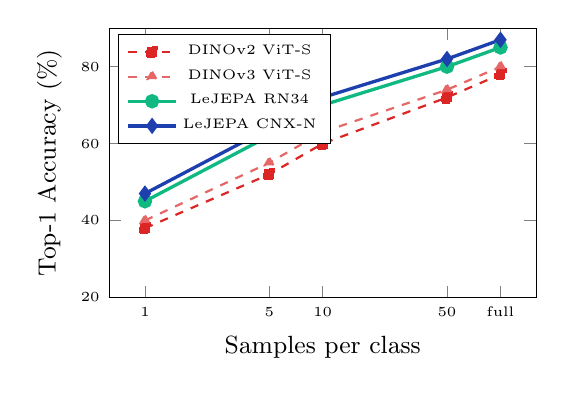
\begin{tikzpicture}
\begin{axis}[
  width=7cm, height=5cm,
  xlabel={\small Samples per class},
  ylabel={\small Top-1 Accuracy (\%)},
  xmode=log, log ticks with fixed point,
  xtick={1,5,10,50,100},
  xticklabels={1,5,10,50,full},
  xticklabel style={font=\tiny},
  yticklabel style={font=\tiny},
  ymin=20, ymax=90,
  legend style={font=\tiny, at={(0.02,0.98)}, anchor=north west},
]
  % DINOv2
  \addplot[bad, thick, mark=square*, dashed, mark size=1.8pt]
    coordinates{(1,38)(5,52)(10,60)(50,72)(100,78)};
  % DINOv3
  \addplot[bad!70, thick, mark=triangle*, dashed, mark size=1.8pt]
    coordinates{(1,40)(5,55)(10,63)(50,74)(100,80)};
  % LeJEPA ResNet-34
  \addplot[good, very thick, mark=*, mark size=2pt]
    coordinates{(1,45)(5,62)(10,70)(50,80)(100,85)};
  % LeJEPA ConvNeXt
  \addplot[primary, very thick, mark=diamond*, mark size=2pt]
    coordinates{(1,47)(5,64)(10,72)(50,82)(100,87)};
  \legend{DINOv2 ViT-S, DINOv3 ViT-S, LeJEPA RN34, LeJEPA CNX-N}
\end{axis}
\end{tikzpicture}

\column{0.42\textwidth}
\textbf{Setup:}
\begin{itemize}\small
  \item Galaxy10: 11,000 anh thien ha, 10 loai
  \item LeJEPA: train truc tiep tren Galaxy10
  \item DINOv2/v3: pretrain tren ImageNet
\end{itemize}
\vspace{8pt}
\begin{alertblock}{Paradigm Shift}
\small Domain-specific SSL (11K anh) \\
$>$ Giant transfer learning \\
(DINOv2 trained on 100M+ imgs)
\end{alertblock}
\vspace{8pt}
\begin{exampleblock}{Implication}
\small Khong can cho Meta/Google ra model cho domain cua ban. 1 GPU + LeJEPA = SOTA tren domain rieng.
\end{exampleblock}
\end{columns}
\takeaway{In-domain SSL > Generic transfer --- ngay ca voi 11K samples}
\end{frame}

% ============================================================
%  SLIDE 28 — Emergent Semantics
% ============================================================
\begin{frame}{Emergent Semantics: LeJEPA Hoc Segment Vat The}
\begin{columns}[c]
\column{0.50\textwidth}
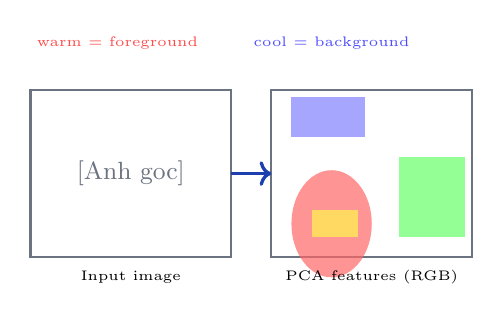
\begin{tikzpicture}[scale=0.85]
  % Original image placeholder
  \draw[thick, neutral] (0,0) rectangle (3,2.5);
  \node[neutral] at (1.5,1.25) {\small [Anh goc]};
  \node[font=\tiny] at (1.5,-0.3) {Input image};
  % PCA visualization placeholder
  \draw[thick, neutral] (3.6,0) rectangle (6.6,2.5);
  % Simulate PCA colors
  \fill[red!60, opacity=0.7] (4.5,0.5) ellipse (0.6cm and 0.8cm);
  \fill[blue!50, opacity=0.7] (3.9,1.8) rectangle (5.0,2.4);
  \fill[green!60, opacity=0.7] (5.5,0.3) rectangle (6.5,1.5);
  \fill[yellow!70, opacity=0.7] (4.2,0.3) rectangle (4.9,0.7);
  \node[font=\tiny] at (5.1,-0.3) {PCA features (RGB)};
  % Arrow
  \draw[->, very thick, primary] (3.0,1.25) -- (3.6,1.25);
  % Legend
  \node[font=\tiny, red!70] at (1.3,3.2) {warm = foreground};
  \node[font=\tiny, blue!70] at (4.5,3.2) {cool = background};
\end{tikzpicture}

\column{0.47\textwidth}
\begin{block}{PCA Feature Visualization}
\small Chieu last-layer features xong $\to$ RGB bang 3 principal components.\\
\textbf{Khong co supervision} --- LeJEPA tu hoc:
\end{block}
\vspace{6pt}
\begin{itemize}\small
  \item \textbf{Mau am} (do/tim): foreground objects
  \item \textbf{Mau lanh} (xanh/vang): background / foliage
  \item Object-background separation \textbf{tu noi len}
\end{itemize}
\vspace{8pt}
\begin{exampleblock}{Video Segmentation}
\small Threshold attention maps cua [CLS] token $\to$ segment + track objects qua video frames.\\
\textbf{Zero segmentation labels} during training.
\end{exampleblock}
\end{columns}
\takeaway{SSL objective dung $\Rightarrow$ semantic structure tu noi len}
\end{frame}

% ============================================================
%  SLIDE 29 — Impact Map
% ============================================================
\begin{frame}{Impact: LeJEPA Mo Ra Nhung Gi?}
\begin{columns}[c]
\column{0.52\textwidth}
\begin{tikzpicture}[scale=0.78]
  % Center
  \node[circle, draw=primary, very thick, fill=lightblue,
        minimum size=1.6cm, font=\small\bfseries, align=center] (center)
        at (0,0) {Le\\JEPA};
  % 5 branches
  \foreach \angle/\lab/\col/\ex in {
    90/Robotics\&World Models/primary!80/V-JEPA--2 DROID,
    162/Scientific ML/good/Galaxy10 Medical,
    234/Edge AI/accent/1-GPU training,
    306/Open Ecosystem/neutral/pip install lejepa,
    18/Academic Theory/primary!50/Provable SSL
  }{
    \node[draw=\col, fill=\col!20, rounded corners=4pt,
          minimum width=2.4cm, minimum height=0.9cm,
          font=\tiny\bfseries, align=center]
          (\angle) at ({2.8*cos(\angle)},{2.8*sin(\angle)}) {\lab};
    \draw[->, thick, \col] (center) -- (\angle);
    \node[font=\tiny, align=center]
      at ({4.5*cos(\angle)},{4.5*sin(\angle)}) {\ex};
  }
\end{tikzpicture}

\column{0.46\textwidth}
\textbf{SSL Timeline:}
\begin{tikzpicture}[scale=0.72]
  \draw[->, very thick, neutral] (-0.3,0) -- (8.5,0);
  \foreach \x/\y/\lab in {
    0/2020/SimCLR,
    1.8/2021/DINO,
    3.6/2023/DINOv2,
    5.4/2024/I-JEPA,
    7.2/2025/LeJEPA
  }{
    \ifnum \x = 0
      \filldraw[neutral] (\x,0) circle (3pt);
    \else \ifnum \x = 72
      \filldraw[primary, very thick] (\x,0) circle (6pt)
        node[above=5pt, primary, font=\small\bfseries] {\lab};
    \else
      \filldraw[neutral] (\x,0) circle (3pt);
    \fi \fi
    \node[font=\tiny, below=4pt] at (\x,0) {\lab};
    \node[font=\tiny, neutral, above=4pt] at (\x,0) {\y};
  }
  \filldraw[primary, very thick] (7.2,0) circle (6pt);
  \node[primary, font=\small\bfseries, above=6pt] at (7.2,0) {$\bigstar$};
  % Annotations
  \node[bad, font=\tiny, below=14pt] at (0,0) {heuristic};
  \node[neutral, font=\tiny, below=14pt] at (1.8,0) {scale};
  \node[neutral, font=\tiny, below=14pt] at (3.6,0) {scale$^2$};
  \node[neutral, font=\tiny, below=14pt] at (5.4,0) {masking};
  \node[good, font=\tiny, below=14pt] at (7.2,0) {\textbf{theory}};
\end{tikzpicture}
\vspace{8pt}
\begin{exampleblock}{}
\footnotesize ``If 2024 was the year of scaling laws, 2025 may be the year we rediscover \textbf{structure}.''
\end{exampleblock}
\end{columns}
\takeaway{LeJEPA dat nen tang cho the he world models tiep theo}
\end{frame}

% ============================================================
%  SLIDE 30 — Usage & Citation
% ============================================================
\begin{frame}{Bat Dau Dung LeJEPA}
\begin{columns}[c]
\column{0.48\textwidth}
\begin{lstlisting}[language=Python, caption={Quick Start}]
import lejepa

# Epps-Pulley univariate test
ep = lejepa.univariate.EppsPulley(
    n_points=17
)

# SIGReg: sliced multivariate test
sigreg = lejepa.multivariate.SlicingUnivariateTest(
    univariate_test=ep,
    num_slices=1024
)

# embeddings: (N, D) tensor
loss = sigreg(embeddings)
loss.backward()
\end{lstlisting}
\vspace{4pt}
\begin{block}{Install}
\texttt{pip install lejepa}\\
\texttt{git clone github.com/rbalestr-lab/lejepa}
\end{block}

\column{0.48\textwidth}
\begin{block}{Ecosystem}
\begin{itemize}\small
  \item \textbf{Backbones:} any timm model (60+)
  \item \textbf{Framework:} PyTorch Lightning via \texttt{stable-pretraining}
  \item \textbf{Eval:} OnlineProbe, OnlineKNN, RankMe callbacks
  \item \textbf{Scale:} DDP-ready, up to 1.8B params
\end{itemize}
\end{block}
\vspace{6pt}
\begin{exampleblock}{Citation}
\scriptsize
\begin{verbatim}
@misc{balestriero2025lejepa,
  title={LeJEPA: Provable and Scalable
    Self-Supervised Learning
    Without the Heuristics},
  author={Balestriero, Randall
    and LeCun, Yann},
  year={2025},
  eprint={2511.08544}
}
\end{verbatim}
\end{exampleblock}
\end{columns}
\end{frame}

% ============================================================
%  SLIDE 31 — Conclusion
% ============================================================
\begin{frame}{Ket Luan}
\begin{columns}[c]
\column{0.55\textwidth}
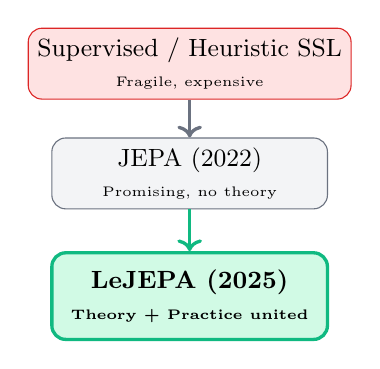
\begin{tikzpicture}[scale=0.82]
  % Journey
  \node[draw=bad, fill=lightred, rounded corners=5pt,
        minimum width=3.5cm, minimum height=0.9cm,
        font=\small, align=center] (s1) at (0,4)
        {Supervised / Heuristic SSL\\{\tiny Fragile, expensive}};
  \node[draw=neutral, fill=lightgray, rounded corners=5pt,
        minimum width=3.5cm, minimum height=0.9cm,
        font=\small, align=center] (s2) at (0,2.3)
        {JEPA (2022)\\{\tiny Promising, no theory}};
  \node[draw=good, very thick, fill=lightgreen, rounded corners=5pt,
        minimum width=3.5cm, minimum height=1.1cm,
        font=\small\bfseries, align=center] (s3) at (0,0.4)
        {LeJEPA (2025)\\{\tiny Theory + Practice united}};
  \draw[->, very thick, neutral] (s1) -- (s2);
  \draw[->, very thick, good] (s2) -- (s3);
\end{tikzpicture}

\column{0.42\textwidth}
\begin{block}{3 Contributions}
\begin{enumerate}\small
  \item[\good{\checkmark}] \textbf{Theory:}\\
  Iso Gaussian uniquely\\
  minimizes downstream risk
  \vspace{4pt}
  \item[\good{\checkmark}] \textbf{Method:}\\
  SIGReg = sliced Epps-Pulley,\\
  $\mathcal{O}(N)$, bounded gradient
  \vspace{4pt}
  \item[\good{\checkmark}] \textbf{Result:}\\
  SOTA tren 60+ archs,\\
  beats DINOv2 in-domain
\end{enumerate}
\end{block}
\end{columns}
\vspace{8pt}
\begin{center}
\Large\itshape\color{primary}
``If 2024 was the year of scaling laws,\\
2025 may be the year we rediscover structure.''
\end{center}
\vfill
\begin{center}
{\large\bfseries Q\&A}
\end{center}
\end{frame}

\end{document}
